\begin{frame}{}
	\tableofcontents
\end{frame}

\section{Section example}
\begin{frame}{Frame title}{Frame subtitle}
	This is the general template for presentations.
	
	\pause
	Use \texttt{\textbackslash pause} command to create steps in your presentation.
	
	\pause
	\begin{block}{Block title}
		Block example
	\end{block}

	\pause
	\begin{alertblock}{Block alert title}
		Block alert example
	\end{alertblock}

	\pause
	\begin{exampleblock}{Block example title}
		Block example example
	\end{exampleblock}
\end{frame}

\begin{frame}{Frame without subtitle}
	This template accepts theorems, examples and proof environments. Here are some examples:
	\begin{theorem}
		There is no largest prime number.
	\end{theorem}
	\begin{proof}
		\begin{enumerate}
			\item<1-> Suppose $p$ were the largest prime number.
			\item<2-> Let $q$ be the product of the first $p$ numbers.
			\item<3-> Then $q + 1$ is not divisible by any of them.
			\item<4-> But $q + 1$ is greater than $1$, thus divisible by some 
			prime number not in the first $p$ numbers.\qedhere
		\end{enumerate}
	\end{proof}
	\uncover<4->{The proof used \textit{reductio ad absurdum}.}
\end{frame}

\section{Texto2}

\begin{frame}{Equations}
	\begin{minipage}[t][\textheight][t]{.5\textwidth}
		\begin{block}{Texto}
			Texto\\
			Texto
		\end{block}
	\end{minipage}%
	\begin{minipage}[t][0.8\textheight][c]{.5\textwidth}
		\begin{equation}
			content...
		\end{equation}
	\end{minipage}
\end{frame}


\begin{frame}{Figures}
	\begin{figure}
		\centering
		\begin{subfigure}[t]{0.5\textwidth}
			\centering
			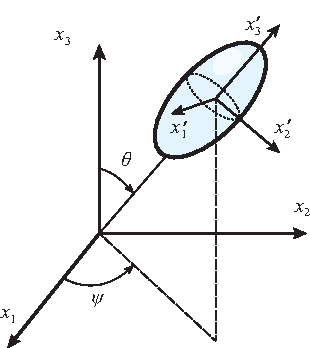
\includegraphics[scale=0.7]{figures/eulerang.pdf}
			\caption{Lorem ipsum}\label{fig:fig1}
		\end{subfigure}%
		~
		\begin{subfigure}[t]{0.5\textwidth}
			\centering
			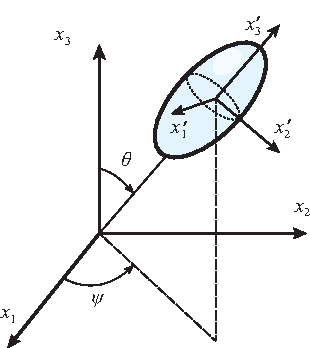
\includegraphics[scale=0.7]{figures/eulerang.pdf}
			\caption{Lorem ipsum}\label{fig:fig2}
		\end{subfigure}
		\caption{Caption \subref{fig:fig1} refered to left figure and \subref{fig:fig2} to refered to right figure.}
		\label{fig:my_label}
	\end{figure}
\end{frame}

\begin{frame}{Tables}
	\begin{table}
		\centering
		\caption{Results of CLT buckling test, obtained from 
		\textcite{pinaNumericalStudyElastic2019} }
		\begin{tabular}{c
						S[table-format=3.0]
						S[table-format=2.0]
						S[table-format=4.0]
						S[table-format=2.2]
						S[table-format=3.1]
						S[table-format=3.2]
						S[table-format=2.2]}
			\toprule
			{\multirow{2}{*}{\makecell{Test\\number}}}
			& {\multirow{2}{*}{\makecell{Width\\/\si{\milli\meter}}}} 
			& {\multirow{2}{*}{\makecell{Total thickness\\/\si{\milli\meter}}}}
			& {\multirow{2}{*}{\makecell{Height\\/\si{\milli\meter}}}}
			& {\multirow{2}{*}{\makecell{$E$\\/\si{\giga\pascal}}}}
			& {\multirow{2}{*}{\makecell{$\lambda_{eff}$}}}
			& {\multirow{2}{*}{\makecell{Critical load\\/\si{\kilo\newton}}}}
			& {\multirow{2}{*}{\makecell{Critical stress\\/\si{\mega\pascal}}}} 
			\\
			&&&&&&&\\\midrule
			1.a   & 150   & 45    & 1000  & 11.65 & 87.8  & 71.85 & 10.64 \\
			1.b   & 150   & 45    & 1000  & 11.65 & 87.8  & 95.31 & 14.12 \\
			2.a   & 150   & 45    & 1980  & 11.65 & 164.6 & 35.76 & 5.3 \\
			2.b   & 150   & 45    & 1990  & 11.65 & 164.6 & 21.12 & 3.13 \\
			3.a   & 150   & 90    & 2000  & 11.29 & 83.1  & 210.14 & 15.57 \\
			3.b   & 150   & 90    & 2000  & 11.29 & 83.1  & 129.24 & 9.57 \\
			3.c   & 150   & 90    & 2000  & 11.29 & 83.1  & 168.98 & 12.52 \\
			3.d   & 150   & 90    & 2000  & 11.29 & 83.1  & 194.89 & 14.44 
			\\\bottomrule
		\end{tabular}%
		\label{tab:CLTresults}%
	\end{table}%
\end{frame}